\documentclass[
    a4paper, aps, twocolumn, floatfix, superscriptaddress, nofootinbib]{revtex4-1}

% It's nice to be able to write your own name
\usepackage[T1]{fontenc}
% Automatic clickable links
\usepackage{hyperref}
% SI-units
\usepackage{siunitx}
% Enhanced math formatting
\usepackage{amsmath}
% Extended math symbols
\usepackage{amssymb}
% Include proof environment
\usepackage{amsthm}
% Import physics package to include bra-ket
\usepackage{physics}
\usepackage{enumerate}
% Import the tensor package for tensors
\usepackage{tensor}
% Include dod and dpd fracs
\usepackage{commath}
% Include font for the identity operator
\usepackage{dsfont}
% Include Tikz
\usepackage{tikz}
% Tikz add-on
\usetikzlibrary{shapes,arrows}
\usetikzlibrary{positioning}
% Several figures in the same figure
\usepackage{subfig}
% Appendix
\usepackage[toc, page]{appendix}

% Macro for latin-letter vectors
\newcommand{\vf}{\mathbf}
% Macro for greek-letter vectors
\newcommand{\vfg}{\boldsymbol}

% Fast macro for real-numbers R
\newcommand{\R}{\mathbb{R}}
% Fast macro for complex-numbers C
\newcommand{\C}{\mathbb{C}}
% Fast macro for polynomial room P
\renewcommand{\P}{\mathbb{P}}
% New command for the identity operator
\newcommand{\1}{\mathds{1}}
% New command for the Lagrangian density
\newcommand{\cL}{\mathcal{L}}
% New command for the Hamiltonian density
\newcommand{\cH}{\mathcal{H}}
% Fast macro for partial differential tensors
\newcommand{\tpl}[1]{\tensor{\partial}{_#1}} % Lower
\newcommand{\tpu}[1]{\tensor{\partial}{^#1}} % Upper
% Fast macro for tensors
\newcommand{\te}[1]{\tensor{#1}}
% Fast macro for commutation and anti-commutation relations
\newcommand{\com}[2]{\left[#1, #2\right]}
\newcommand{\acom}[2]{\left\{#1, #2\right\}}

% Macros for writing auto-sized paranthesis, brackets and braces
\newcommand{\para}[1]{\left(#1\right)}
\newcommand{\brak}[1]{\left[#1\right]}
\newcommand{\brac}[1]{\left\{#1\right\}}

% Macro for creating orbital bra-ket's, i.e., bra-ket with paranthesis edges
\newcommand{\obra}[1]{( #1 \lvert}
\newcommand{\oket}[1]{\rvert #1 )}
\newcommand{\obraket}[2]{( #1 \lvert #2 )}

% Macro for expectation value
\newcommand{\expv}[1]{\langle #1 \rangle}

\newcommand{\half}{\frac{1}{2}}




\begin{document}

\title{Variational Monte Carlo on bosonic systems}
\author{Winther-Larsen, Sebastian Gregorius}
\affiliation{University of Oslo}
\author{Schøyen, Øyvind Sigmundson}
\affiliation{University of Oslo}
\date{\today}

\begin{abstract}
    Something very abstract and clever should go here.
    \begin{figure}[h!]
    \centering
    
\includegraphics[width=0.7\textwidth]{loopholes.jpg}
\end{figure}
\end{abstract}

\maketitle
\tableofcontents

%\begin{widetext}

%\end{widetext}

\section{Introduction}
    We will in this project study the Variational Monte Carlo (VMC) method, and
    use it to evaluate the ground state energy of a trapped, hard sphere Bose
    gas. \cite{dubois2001bose} \cite{nilsen2005vortices}

\section{Theory}
    To model the trapped bosonic gas particles we use the potential
    \begin{align}
        V_{\text{ext}}(\vf{r})
        &=
        \begin{cases}
            \half m\omega^2r^2 & (\text{S}), \\
            \half m \bigl[
                \omega^2(x^2 + y^2) + \omega_z^2z^2
            \bigr] & (\text{E}),
        \end{cases}
    \end{align}
    where we can choose between a spherical (S) or an elliptical (E) harmonic
    trap. The two-body Hamiltonian of the system is given by
    \begin{align}
        H = \sum_{i = 1}^{N}h(\vf{r}_i) + \sum_{i < j}^{N}w(\vf{r}_i, \vf{r}_j),
    \end{align}
    where the single particle one body operator, $h$, is given by
    \begin{align}
        h(\vf{r}_i) = -\frac{\hbar^2}{2m}_i^2
        + V_{\text{ext}}(\vf{r}_i),
    \end{align}
    (we assume equal mass)
    and the two-body interaction operator, $w$, is
    \begin{align}
        w(\vf{r}_i, \vf{r}_j)
        = \begin{cases}
            \infty & |\vf{r}_i - \vf{r}_j| \leq a, \\
            0 & |\vf{r}_i - \vf{r}_j| > a,
        \end{cases}
    \end{align}
    where $a$ is the hard sphere of the particle. The trial wavefunction,
    $\ket{\Psi_T}$, we will
    be looking at is given by
    \begin{align}
        \Psi_T(\vf{r})
        &= \Phi_T(\vf{r})
        \prod_{j < k}^N f(a, \vf{r}_j, \vf{r}_k) \\
        &= \Biggl(
            \prod_{i = 1}^N g(\alpha, \beta, \vf{r}_i)
        \Biggr)
        \prod_{j < k}^N f(a, \vf{r}_j, \vf{r}_k),
        \label{eq:initial_trial_wavefunction}
    \end{align}
    where $\alpha$ and $\beta$ are variational parameters and
    \begin{align}
        \vf{r} = (\vf{r}_1, \vf{r}_2, \dots, \vf{r}_N, \alpha, \beta).
    \end{align}
    Here $g$ are the single particle wavefunctions given by
    \begin{align}
        g(\alpha, \beta, \vf{r}_i)
        = \exp\bigl[
            -\alpha(x_i^2 + y_i^2 + \beta z_i^2)
        \bigr] \equiv \phi(\vf{r}_i),
    \end{align}
    and $\ket{\Phi_T}$ the \textit{Slater permanent} consisting of the $N$ first
    single particle wavefunctions, and the correlation wavefunction, $f$, given
    by
    \begin{align}
        f(a, \vf{r}_j, \vf{r}_k)
        &=
        \begin{cases}
            0 & |\vf{r}_j - \vf{r}_k| \leq a, \\
            \Bigl(
                1 - \frac{a}{|\vf{r}_j - \vf{r}_k|}
            \Bigr) & |\vf{r}_j - \vf{r}_k| > a.
        \end{cases}
    \end{align}
    We will for brevity use the notation $\phi(\vf{r}_i) = \phi_i$ and $r_{jk} =
    |\vf{r}_j - \vf{r}_k|$.

    \subsection{Local energy}
        As the many-body wavefunction creates a very large configuration space,
        where much of the wavefunction is small, we use the Metropolis algorithm
        in order to move towards regions in configuration space with
        ``sensible'' values. We define the \textit{local energy}, $E_L{\vf{r}}$,
        by
        \begin{align}
            E_L(\vf{r})
            &= \frac{H\Psi_T(\vf{r})}{\Psi_T(\vf{r})}.
        \end{align}
        If $\ket{\Psi_T}$ is an exact eigenfunction of the Hamiltonian, $E_L$
        will be constant. The closer $\ket{\Psi_T}$ is to the exact wave
        function, the less variation in $E_L$ as a function of $\vf{r}$ we get.
        One of the most computationally intensive parts of the VMC algorithm
        will be to compute $E_L$. We therefore find an analytical expression for
        $E_L$ in terms of the trial wavefunction.

    \subsection{The drift force}
        A disadvantage in the use of the brute-force Metropolis algorithm is
        that we might be spending much computational resources in an
        uninteresting part of configuration space. To make smarter moves we will
        use the Metropolis-Hastings algorithm (which will be discussed in due
        time). This algorithm is dependent on the drift force of the system.
        \begin{align}
            \vf{F}(\vf{r})
            &=
            \sum_{k = 1}^N
            \vf{F}_k(\vf{r})
            =
            \sum_{k = 1}^N
            \frac{2\nabla_k\Psi_T(\vf{r})}{\Psi_T(\vf{r})}.
            \label{eq:drift_force}
        \end{align}
        Using this expression we are able to move towards parts of
        configuration space where the gradient increases or decreases yielding a
        better choice of movements. We will mainly be interested in the drift
        force of a single particle $k$.

\section{Non-interacting harmonic oscillators}
    We start by looking at a simple system of non-interacting harmonic
    oscillators. That is, where $a = 0$ and $\beta = 1$. We thus get the trial
    wavefunction
    \begin{align}
        \Psi_T(\vf{r})
        = \Phi_T(\vf{r})
        = \prod_{i = 1}^N \exp\bigl[
            -\alpha |\vf{r}_i|^2
        \bigr],
    \end{align}
    where $|\vf{r}_i| = r_i$. As $a = 0$ the interaction term,
    $w(\vf{r}_i, \vf{r}_j)$, vanishes and the Hamiltonian is given by
    (in the spherical case)
    \begin{align}
        H &= \sum_{i = 1}^N h(\vf{r}_i)
        = \sum_{i = 1}^N \Biggl(
            -\frac{\hbar^2}{2m}\nabla_i^2
            + \half m \omega^2 r_i^2
        \Biggr).
    \end{align}
    To find the drift force and the local energy we have to compute the gradient
    and the Laplacian of the trial wavefunction. The gradient is given by
    \begin{align}
        \nabla_k\Psi_T(\vf{r})
        &= -2\alpha \vf{r}_k\Psi_T(\vf{r}),
    \end{align}
    whereas the Laplacian yields
    \begin{align}
        \nabla^2_k\Psi_T(\vf{r})
        &= \big(-2d\alpha + 4\alpha^2 r_k^2\bigr)\Psi_T(\vf{r}),
    \end{align}
    where $d$ is the dimensionality of the problem determined by
    $\vf{r}_k \in \mathbb{R}^d$. We can thus use the gradient to find an
    expression for the drift force for particle $k$.
    \begin{align}
        \vf{F}_k(\vf{r})
        &= -2\alpha\vf{r}_k.
    \end{align}
    Using the Laplcian we can compute the kinteic term in the expression for the
    local energy. We get
    \begin{align}
        E_L(\vf{r})
        &=
        \sum_{i = 1}^N
        \Biggl(
            -\frac{\hbar^2}{2m}
            \bigl[
                -2d\alpha + 4\alpha^2 r_i^2
            \bigr]
            + \half m\omega^2 r_i^2
        \Biggr).
    \end{align}
    In natural units, with $\hbar = c = m = 1$, this reduces to
    \begin{align}
        E_L(\vf{r})
        &=
        \alpha dN
        + \biggl(
            \half\omega^2
            - 2\alpha^2
        \biggr)
        \sum_{i = 1}^N r_i^2.
        \label{eq:closed_form_natural_units_local_energy}
    \end{align}
    It is worth noting that for $\alpha = \half\omega$ ($\alpha$ is required to
    be positive) we will find a stable value which turns out to be the exact
    energy minimum. This happens as the entire sum over all the random walkers
    disappears.

    \subsection{Exact variational energy}
        As the system is non-interacting and consisting of Gaussians we can
        find an expression for the exact energy as a function of the
        variational parameter $\alpha$, i.e.,
        \begin{align}
            E(\alpha)
            &=
            \frac{\bra{\Psi_T}H\ket{\Psi_T}}{\bra{\Psi_T}\ket{\Psi_T}}.
        \end{align}

        % TODO: Add the computation of this expression
        The final result for the energy is
        \begin{align}
            E(\alpha)
            &=
            \left(
                \frac{\hbar^2 \alpha}{2m}
                + \frac{m\omega^2}{8\alpha}
            \right)dN.
        \end{align}
        By minimizing this expression, i.e., finding the derivative of the
        energy with respect to $\alpha$ and equating this to zero, yields the
        expected minimum of variational energy to be
        \begin{align}
            \dod[]{E(\alpha)}{\alpha} = 0
            \implies
            \alpha_0 = \frac{m\omega}{2\hbar},
        \end{align}
        which in natural units reduces to $\alpha_0 = \half\omega$. The energy at
        this value of $\alpha$ (in natural units) is then
        \begin{align}
            E(\alpha_0)
            &=
            \frac{\omega dN}{2}.
        \end{align}


\section{Interacting hard sphere bosons}
    Moving to the full system allowing $\beta$ to vary and setting $a
    \neq 0$ we can write the trial wavefunction as
    \begin{align}
        \Psi_T(\vf{r})
        &=
        \Phi_T(\vf{r})
        J(\vf{r}),
    \end{align}
    where $\ket{\Phi_T}$ is the same Slater permanent as in
    \autoref{eq:initial_trial_wavefunction} and $J(\vf{r})$ is the
    \textit{Jastrow factor} given by
    \begin{align}
        J(\vf{r})
        &=
        \exp\Biggl(
            \sum_{j < l}^N u(r_{jl})
        \Biggr),
    \end{align}
    where $r_{jk} = |\vf{r}_j - \vf{r}_k|$ and
    \begin{align}
        u(r_{jk}) = \ln\bigl[f(a, \vf{r}_j, \vf{r}_k)\bigr].
    \end{align}
    To further shorten the notation we will use $u_{jk} = u(r_{jk})$. Computing
    the gradient of the wavefunction we get
    \begin{align}
        \nabla_k\Psi_T(\vf{r})
        &=
        \Bigl[
            \nabla_k
            \Phi_T(\vf{r})
        \Bigr]
        J(\vf{r})
        + \Phi_T(\vf{r})
        \nabla_k J(\vf{r}).
    \end{align}
    The gradient of the Slater permament for particle $k$ is given by
    \begin{align}
        \nabla_k
        \Phi_T(\vf{r})
        &=
        \nabla_k\phi_k
        \prod_{i \neq k}^N\phi_i
        = \frac{\nabla_k\phi_k}{\phi_k}
        \Phi_T(\vf{r}).
    \end{align}
    The gradient of the Jastrow factor is given by
    \begin{align}
        \nabla_k J(\vf{r})
        &=
        J(\vf{r})
        \nabla_k\sum_{m < n}^N u_{mn} \\
        &= J(\vf{r})
        \Biggl(
            \sum_{m = 1}^{k - 1}\nabla_k u_{mk}
            \sum_{n = k + 1}^N\nabla_k u_{kn}
        \Biggr)
        \\
        &=
        J(\vf{r})
        \sum_{m \neq k}^N\nabla_k u_{km},
    \end{align}
    where the gradient of the interaction term splits the antisymmetric
    sum into two parts. As $r_{ij} = r_{ji}$ we can combine these sums
    into a single sum. This in total yields the gradient
    \begin{align}
        \nabla_k\Psi_T(\vf{r})
        &=
        \Biggl(
            \frac{\nabla_k\phi_k}{\phi_k}
            + \sum_{m \neq k}^N
            \nabla_k u_{km}
        \Biggr)
        \Psi_T(\vf{r}).
        \label{eq:gradient_full_wavefunction}
    \end{align}

    The Laplcian of the trial wavefunction is found by finding the divergence of
    \autoref{eq:gradient_full_wavefunction}.
    \begin{align}
        \nabla_k^2\Psi_T(\vf{r})
        &=
        \Biggl(
            \nabla_k\Biggl[
                \frac{\nabla_k\phi_k}{\phi_k}
            \Biggr]
            +
            \sum_{m \neq k}^N \nabla_k^2 u_{km}
        \Biggr)\Psi_T(\vf{r})
        \\
        &\qquad
        +
        \Biggl(
            \frac{\nabla_k\phi_k}{\phi_k}
            + \sum_{m \neq k}^N
            \nabla_k u_{km}
        \Biggr)^2
        \Psi_T(\vf{r}),
    \end{align}
    where the squared term came from taking the gradient of the trial
    wavefunction.  To further simplify we divide by the trial
    wavefunction. This yields
    \begin{align}
        \frac{\nabla_k^2\Psi_T(\vf{r})}{\Psi_T(\vf{r})}
        &=
        \frac{\nabla_k^2\phi_k}{\phi_k}
        + 2\frac{\nabla_k\phi_k}{\phi_k}
        \sum_{m \neq k}\nabla_k u_{km}
        \nonumber \\
        &\qquad
        + \sum_{m\neq k}^N\nabla_k^2 u_{km}
        + \Biggl(
            \sum_{m \neq k}^N\nabla_k u_{km}
        \Biggr)^2.
    \end{align}
    To go from here we have to find the gradient and the Laplacian of
    the single particle functions, $\phi_k$, and the interaction
    functions $u_{km}$. For the single particle functions we use
    Cartesian coordinates when finding the derivatives whereas we for
    the interaction functions will use spherical coordinates and do a
    variable substitution. Beginning with the gradient of the single
    particle functions we get
    \begin{align}
        \nabla_k\phi_k
        &=
        \nabla_k\exp\bigl[
            -\alpha(x_k^2 + y_k^2 + \beta z_k^2)
        \bigr] \\
        &=
        -2\alpha
        (x_k\vf{e}_i + y_k\vf{e}_j + \beta z_k\vf{e}_k)
        \phi_k.
    \end{align}
    Note that the subscripts on the unit vectors $\vf{e}_i$ are
    \textit{not} the same as the subscripts used for its components. The
    Laplacian yields
    \begin{align}
        \nabla_k^2\phi_k
        &=
        \Bigl[
            -2\alpha
            \big(
                d - 1 + \beta
            \bigr)
            \nonumber \\
            &\qquad
            + 4\alpha^2
            \bigl(
                x_k^2 + y_k^2 + \beta^2z_k^2
            \bigr)
        \Bigr]
        \phi_k,
    \end{align}
    with $d$ as the dimensionality of the problem.
    In order to derive the interaction functions we have to do a
    variable substitution using $r_{km} = |\vf{r}_k - \vf{r}_m|$. We can
    then rewrite the $\nabla_k$-operator as
    \begin{align}
        \nabla_k
        &=
        \nabla_k
        \dpd[]{r_{km}}{r_{km}}
        =
        \nabla_k r_{km} \dpd[]{}{r_{km}}
        \\
        &=
        \frac{\vf{r}_k - \vf{r}_m}{r_{km}}\dpd[]{}{r_{km}}.
    \end{align}
    Applying this version of the $\nabla_k$-operator to $u_{km}$ yields
    \begin{align}
        \nabla_k u_{km}
        &=
        \frac{\vf{r}_k - \vf{r}_m}{r_{km}}
        \dpd[]{u_{km}}{r_{km}}.
    \end{align}

    \begin{widetext}
        For the Laplacian we switch a little back and forth between the
        two ways of representing the $\nabla_k$-operator. We thus get
        \begin{align}
            \nabla_k^2 u_{km}
            &=
            \frac{\nabla_k \vf{r}_k}{r_{km}}\dpd[]{u_{km}}{r_{km}}
            + \Biggl[
                \nabla_k \frac{1}{r_{km}}
            \Biggr]
            (\vf{r}_k - \vf{r}_m)\dpd[]{u_{km}}{r_{km}}
            + \frac{\vf{r}_k - \vf{r}_m}{r_{km}}
            \nabla_k \dpd[]{u_{km}}{r_{km}} \\
            &= \frac{d}{r_{km}}\dpd[]{u_{km}}{r_{km}}
            - \frac{(\vf{r}_k - \vf{r}_m)^2}{r_{km}^3}
            \dpd[]{u_{km}}{r_{km}}
            + \frac{(\vf{r}_k - \vf{r}_m)^2}{r_{km}^2}
            \dpd[2]{u_{km}}{r_{km}} \\
            &=
            \frac{d - 1}{r_{km}}\dpd[]{u_{km}}{r_{km}}
            + \dpd[2]{u_{km}}{r_{km}},
        \end{align}
        where $d$ is again the dimensionality of the problem. In total
        we can state an intermediate version of the Laplacian occuring
        in the local energy as
        \begin{align}
            \frac{\nabla_k^2\Psi_T(\vf{r})}{\Psi_T(\vf{r})}
            &=
            \frac{\nabla_k^2\phi_k}{\phi_k}
            + 2\frac{\nabla_k\phi_k}{\phi_k}
            \sum_{m \neq k}^N
            \frac{\vf{r}_k - \vf{r}_m}{r_{km}}
            \dpd[]{u_{km}}{r_{km}}
            + \sum_{m\neq k}^N
            \Biggl(
                \frac{d - 1}{r_{km}}\dpd[]{u_{km}}{r_{km}}
                + \dpd[2]{u_{km}}{r_{km}}
            \Biggr)
            \nonumber \\
            &\qquad
            +
            \sum_{m, n \neq k}^N
            \frac{\vf{r}_k - \vf{r}_m}{r_{km}}
            \frac{\vf{r}_k - \vf{r}_n}{r_{kn}}
            \dpd[]{u_{km}}{r_{km}}
            \dpd[]{u_{kn}}{r_{kn}}.
        \end{align}
    \end{widetext}
    Moving on to the derivatives of the interaction terms, $u_{km}$, to
    get an explicit expression for the Laplacian.
    \begin{align}
        \dpd[]{u_{km}}{r_{km}}
        &=
        \frac{a}{r_{km}(r_{km} - a)},
        \\
        \dpd[2]{u_{km}}{r_{km}}
        &= \frac{a^2 - 2ar_{km}}{r_{km}^2(r_{km} - a)^2}.
    \end{align}
    The local energy and the drift force can now be found by combining these
    expressions. For brevity, we will not write out the explicit expressions as
    these will be called by separated functions in our programs.

    \subsection{Scaling the system}
        We now introduce a scaled distance $\vf{r}' = \vf{r}/a_{\text{ho}}$
        \cite{dubois2001bose}, where
        \begin{align}
            a_{\text{ho}}
            &=
            \sqrt{\frac{\hbar}{m\omega}}.
        \end{align}
        We can then rewrite the Hamiltonian for the elliptic potential in terms
        of this new distance. By doing a variable substitution for each
        direction in the Laplace operator we get
        \begin{align}
            \nabla_k^2
            &=
            \frac{1}{a_{\text{ho}}^2}{\nabla_k'}^2.
        \end{align}

        Looking at the one-body part of the Hamiltonian we get
        \begin{align}
            H
            &=
            \sum_{k = 1}^N
            \brac{
                -\frac{\hbar^2}{2m}\nabla_k^2
                + \half m\brak{
                    \omega^2(x_k^2 + y_k^2)
                    + \omega_z^2 z_k^2
                }
            }
            \\
            &=
            \frac{\hbar\omega}{2}
            \sum_{k = 1}^N
            \brac{
                -{\nabla_k'}^2
                +
                \brak{
                    {x_k'}^2 + {y_k'}^2 + \lambda^2{z_k'}^2
                }
            },
        \end{align}
        where we have introduced the dimensionless frequency $\lambda =
        \omega_z/\omega$. The single particle functions also gets a scaling
        factor
        \begin{align}
            \phi_k
            &=
            \exp\brak{
                -\frac{\alpha\hbar}{m\omega}
                ({x_k'}^2 + {y_k'}^2 + \beta^2{z_k'}^2)
            }
            \equiv
            \phi(\vf{r}_k').
        \end{align}
        The correlation wavefunction and the interaction potential remain the
        same, but using the scaled hard core sphere radius $a/a_{\text{ho}} =
        0.0043$. For brevity we will remove the ticks on the variables.


\section{Algorithms}
    In the project we rely on a Monte Carlo approach of random sampling to
    obtain numerical results.  We simulate random walks over a volume in order
    to find optimal parameters in our trial wavefunctions.  The most common of
    such methods, which we make use of herein, is the Metropolis-Hastings
    algorithm.

    \subsection{The Metropolis-Hastings Algorithm}
        The Metropolis-Hastings algorithm can in our particular situation be
        condensed down to the following steps:

        \begin{enumerate}
            \item The system is initialised by a certain number $N$ of randomly
                generated positions, or particles. This allows us to evaluate
                the wavefunction at these points and compute the local energy
                $E_L$.

            \item The initial configuration is changed by setting a new position
                for one of these particles. The particle is picked at random.

            \item A ratio between new wavefunction density and the previous
                (initial) density is computed and compared to a random number.
                This acceptance probability decides if the particle move is
                rejected or accepted.  The particle is only allowed to move a
                predetermined step length.

            \item If the particle movement is accepted and the local energy
                $E_L$ is computed for the new system.

            \item Repeat steps until convergence and an optimum is reached.

        \end{enumerate}

        The algorithm described above can be applied in an "exhaustive" search
        of the parameter space in order to find the optimal parameters.  Whether
        a proposed move is accepted or not is determined by a transition
        probability and the acceptance probability.  The strength of the
        algorithm is that the transition algorithm need not be known. For
        example, the simplest case is to accept the new state, i.e., the new
        position for the random walker, if the ratio
        \begin{align}
            q(\vf{r}_{i + 1}, \vf{r}_i)
            &=
            \frac{\left|\Psi_T(\vf{r}_{i + 1})\right|^2}
            {\left|\Psi_T(\vf{r}_{i})\right|^2},
        \end{align}
        where $\vf{r}_{i + 1}$ are all the positions at step $i + 1$, is greater
        than a uniform probability $p \in [0, 1)$.

        \subsubsection{Importance Sampling}
            A problem with the naïve Metropolis-Hastings sampling approach is
            that the sampling of position space is done with no regard for where
            we are likely to find a particle. This problem can be remedied
            through \emph{importance sampling}.  It is reasonable to assume that
            the particles we erratically scatter in space are prone to movement
            towards the peaks of the probability density as dictated by the wave
            function. Consider therefore the Fokker-Planck equation,
            \begin{align}
                \dpd[]{\Psi_T}{t}
                &=
                D \nabla\cdot
                \left(
                    \nabla
                    - \vf{F}
                \right) \Psi_T,
                \label{eq:fokker_planck}
            \end{align}
            which describes the evolution in time of a probability density
            function. In our case this is the trial wavefunction $\Psi_T$.
            Originaly an equation that models diffusion, we have a diffusion
            term $D$ and the drift force \autoref{eq:drift_force}. In our case
            the diffusion term $D$ is simply $1/2$ from the kinetic energy (in
            natural units).

            We use the Langevin equation to find the new position of the
            particle.
            \begin{align}
                \dpd[]{\vf{r}}{t}
                &=
                D\vf{F}(\vf{r}) + \vfg{\eta},
                \label{eq:langevin}
            \end{align}
            where $\vfg{\eta}$ is a uniformly distributed stochastic variable
            for each dimenion.  Solving Langevin's equation by Euler's method
            gives a recursive relation for the subsequent new positions of a
            particle.
            \begin{align}
                \vf{r}_{i + 1}
                &=
                \vf{r}_i + D\vf{F}(\vf{r}_i)\Delta t
                + \vfg{\xi}\sqrt{\Delta t},
            \end{align}
            for a given time step $\Delta t$
            \footnote{
                Bear in mind that \autoref{eq:langevin} is only valid as $\Delta
                t \to 0$, a property stemming from the use of Euler's method.
            }
            and a normally distributed stochastic variable $\vfg{\xi}$.

            Now we need to change the acceptance probability of the metropolis
            algorithm to something that takes the new sampling method into
            account.
            \begin{align}
                q(\vf{r}_{i + 1}, \vf{r}_i)
                &=
                \frac{
                    G(\vf{r}_{i + 1}, \vf{r}_{i}, \Delta t)
                    \left|\Psi_T(\vf{r}_{i + 1})\right|^2
                }
                {
                    G(\vf{r}_{i}, \vf{r}_{i + 1}, \Delta t)
                    \left|\Psi_T(\vf{r}_{i})\right|^2
                },
            \end{align}
            where $G$ is the Green's function of the Fokker-Planck equation
            given by
            \begin{align}
                G(\vf{r}_{i + 1}, \vf{r}_i, \Delta t)
                &=
                \exp\Biggl(
                    -\frac{\bigl[
                        \vf{r}_{i + 1}
                        - \vf{r}_{i}
                        - D\vf{F}(\vf{r}_i)\Delta t
                    \bigr]^2}{4D\Delta t}
                \Biggr)
                \nonumber \\
                &\qquad
                \times
                \frac{1}{(4\pi D\Delta t)^{dN/2}},
            \end{align}
            where $d$ is the dimensionality.

    \subsection{Statistical Analysis}
        If the results of the metropolis sampling were completely uncorrelated,
        it would be enough to compute the standard deviation in a familiar way,
        \begin{equation}
            \sigma = \sqrt{\frac{1}{N}(\ev{E^2_L} - \ev{E_L}^2},
            \label{eq:standard_deviation}
        \end{equation}
        where $N$ is the number of samples, or Monte-Carlo cycles, in the experiment.
        However, it is reasonable to assume that the data we are dealing with in this
        study is liable to suffer from \emph{autocorrelation} and \autoref{eq:standard_deviation}
        does not hold. The prevailing
        definition of autocorrelation in a data stream or signal is correlation
        between a delay of the signal and the original signal. One would be interested to find the
        delay, or lag, in the signal at which the "self-correlation" is highest. We refer to this
        spacing as $d$, and define the following correlation function,
        \begin{equation}
            f_d = \frac{1}{n -d} \sum_{k=1}^{n-d} (x_k - \bar{x}_n)(x_{k+d} - \bar{x}_n).
            \label{eq:correlation_f_d}
        \end{equation}
        The keen reader would have noticed that the function $f_d$ in \autoref{eq:correlation_f_d}
        would be equal to the sample variance for $d=0$. We can now define the \emph{autocorrelation function}
        \begin{equation}
            \kappa_d = \frac{f_d}{\text{Var}(x)},
            \label{eq:autocorrelation_function}
        \end{equation}
        which is equal to $1$ if the data exhibits no autocorrealtions, equating to $d=0$. From the autocorrelation
        function (\ref{eq:autocorrelation_function}) we in turn define the \emph{autocorrelation time},
        \begin{equation}
            \tau = 1 + 2 \sum_{d=1}^{n-1}\kappa_d,
        \end{equation}
        notice that the autocorrelation time is $1$ for a correlation free experiment.

        We are now able to make a correction to the expression for the standard deviation
        improving on \autoref{eq:standard_deviation} by taking correlation into account,
        \begin{equation}
            \sigma =\sqrt{\frac{1 + 2\tau / \Delta t}{N}(\ev{E^2_L} - \ev{E_L}^2)},
        \end{equation}
        where $\Delta t$ is the time between each sample. The main problem at this point is to
        find $\tau$, which we do not know for any given system and it is generally very expensive to
        compute. In order to find a good estimate of $\tau$ we use a procedure called \emph{blocking}.

        \subsubsection{Blocking}
        In the method of blocking we group the samples into blocks of increasing size. If one where to compute
        the standard deviation for each block, one should see the variance increase with the block size.
        The standard deviation would only increase up to a certain point, from whence it would stay
        almost constant. What is happening is that we have reached a point where a particular
        sample from one block is no longer correlated with a corresponding sample from an adjacent block.
        The block size for this point of convergence now functions as an estimate for the autocorrelation
        time $\tau$.
        
     	Instead of going by this "manual" method of looking at charts, we will construct a test statistic and
     	let the computer do the necessary considerations in a more "automatic way.
        
        The easiest way to do this is by use of the \emph{automatic blocking scheme}, nicely illustrated 
        with a flow chart in \autoref{fig:blocking}. The input parameter for the method is an array of the 
        local energies, but it can be any array of time series data, which is why it is herein referred to as
        $\mathbf{X}$. Any array of sequential data, where any particular data point depends on the previous
        data point inhibits all attributes of a time series. Our array of local energies is therefor most definitely 
        a time series. 
        
		From $\mathbf{X}$ we compute the variance and sample covariance between the series itself and a 
		one-point lag of the series. This covariance is usually referred to as the first order autocovariance.
		\begin{equation}
			\gamma_i = \frac{1}{n}
				\left(\sum_{k=1}^n\left((\mathbf{X}_i)_k - (\bar{\mathbf{X}}_i)_k\right)\right)
				\left(\sum_{k=0}^{n-1}\left((\mathbf{X}_i)_k - (\bar{\mathbf{X}}_i)_k\right)\right).
		\end{equation}
		
		Now we "block"! The next step is to perform a transformation of the our time series $\mathbf{x}_i$, where
		we end up with an array that is half the length of the original time series,
		\begin{equation}
			(\mathbf{X}_i)_k = \frac{1}{2}\left((\mathbf{X}_i)_{2k-1} + (\mathbf{X}_i)_{2k} \right).
		\end{equation}
		This process is were the term "blocking" stems from. There are a number of ways to perform the blocking -
		we could have picked the data points used in the new ($i+1$) array randomly, or more orderly. Here we we have
		picked them sequentially. We have obtained $\frac{n}{2}$ new "primed" stochastic variables. Assuming that the
		reader is playing close attention, it is now needless to say that it is much easier to perform these sequential
		blocking steps if we have an array of length $n= 2^d$, where $d$ is integer. Otherwise, problems would arise
		because one would have arrays of different lengths when the original array is "split in two". The ailment is
		easy to remedy by excluding an observation from the longest resulting array after splitting. 
		
		For each new time series $\mathbf{X}_{i+1}$ a new sample variance and sample covariance is computed.
		The blocking transformation is allowed to continue until we are we run out of data, i.e. the length
		of $\mathbf{X}_i < 2$. In other words, there is only a single number left. We now compute a test statistic,
		\begin{equation}
			M_j = \sum_{k=j}^{d-1} n_k \frac{\left[(n_k - 1)\frac{s^2_k}{n_k^2} y \gamma_k(1)\right] ^2}{s_k^4}.
		\end{equation}
		As luck would have it, this number $M$ is   $\chi^2$-distributed. The following step would be to look up a 
		statistical table and find the first $k$, such that $M_k \leq q_{d-k}(1-\alpha)$, where $q$ is the statistical
		limit and $\alpha$ is  the significance level that your hear desires. Finally, the correct sample standard deviation 
		is $\frac{s_k^2}{n_k}$. Again, see \autoref{fig:blocking} for a summary of the algorithm. 
		        
        % Flow chart for description of automatic blocking algorithm
		\begin{figure}
			\centering
        
        		% Defining blocks of flowchart
        		\tikzstyle{decision} = [diamond, draw, fill=blue!20, 
   			 	text width=5em, text badly centered, node distance=3cm, inner sep=0pt]
			\tikzstyle{block} = [rectangle, draw, fill=blue!20, 
    				text width=11em, text centered, rounded corners, minimum height=4em]
			\tikzstyle{line} = [draw, -latex']
    			
    			% Actual figure
    			\begin{tikzpicture}[node distance = 2.2cm, auto]
    			
    				% Nodes
    				\node [block] (init) {Start with $\mathbf{X}_i$, $i=0$};
    				\node [block, below of=init] (variance) {Compute variance and autocovariance of $\mathbf{X}_i$, $s_i$ and $\gamma_i$};
    				\node [block, below of=variance] (transform) 
    					{Transform data $(\mathbf{X}_{i+1})_k = \frac{1}{2}\left((\mathbf{X})_i)_{2k-1} + (\mathbf{X}_i)_{2k} \right)$};
    				\node [block, right=1.5cm of transform] (i+1) {Next iteration: $i = i + 1$.} ;
    				\node [decision, below of = transform] (x_size) {Length of $\mathbf{X}_{i + 1} \geq 2$ ? }; 
    				\node [block, below of=x_size] (m_test) {Compute test statistic $M_j$ from $s_j$ and $\gamma_j$ for all $j$.};
    				\node [block, below of=m_test] (magic_numbers) {Find first $k$ so that $M_k \leq q_{d-k}(1-\alpha)$};
    				\node [block, below of=magic_numbers] (return) {Return $s_k^2/n_k$};
    			
    				% Edges
    				\path [line] (init) -- (variance);
    				\path [line] (variance) -- (transform);
    				\path [line] (transform) -- (x_size);
    					\path [line] (x_size) -| node [near start] {yes} (i+1);
    					\path [line] (i+1) |- (variance);
    				\path [line] (x_size) -- node [near start] {no} (m_test);
    				\path [line] (m_test) -- (magic_numbers);
    				\path [line] (magic_numbers) -- (return);
    			\end{tikzpicture}
    			\caption{Flow chart depicting the automatic blocking method for finding a better estimate for sample variance.}
    			\label{fig:blocking}
		\end{figure}
		
		\subsection{Gradient Descent}
		
		Scanning the entire space of variational parameters can be a somewhat despairing task. To aid us in the search we
		therefore implement the method of gradient descent\footnote{Also known as steepest descent, easily confused
		with the steepest descent method for integation.}. In any optimum we generally have that the derivative should equal
		zero. In our case, we want to find the minimum of the expected local energy with respect to some variational
		parameter $\alpha$, so that
		\begin{equation}
			\nabla_\alpha \expval{E_L(\mathbf{R}; \alpha)} = 0.
		\end{equation}	
		The foundation for  the method of gradient descent lies in the fact that some analytic
		\footnote{We use the term analytic quite recklessly.} function $F(\alpha)$ decreases fastest in the direction
		of $-\nabla_\alpha F(\alpha)$. This means that we could eventually get to an ensuing minimum by trailing along the
		pathway of the following recursive relation,
		\begin{equation}
			\alpha_{k+1} = \alpha_k - \gamma \nabla_{\alpha k} F(\alpha_k).
		\end{equation}
		If $\gamma$ is small enough we should have $f(\alpha_k) \geq F(\alpha_{k+1})$ for all $k$ and hopefully we will
		experience convergence to the desired minimum. 
		
		For our special case : INSERT DERIVATION OF LOCAL ENERGY derivative wrt alpha??

\section{Results}

    \subsection{Non-Interacting Systems}
    Initially we are interested in seeing how our implementation performs and to what extent it functions properly.
    the logical thing to do would be to look at a non-interacting system with a simple Gaussian wavefunction and
    harmonic oscillator potential. Such a system has a simple closed-form analytic solution\footnote{A fact that every
    undergraduate physics student should be well aware of after finishing their first course in quantum physics}, 
    which is further simplified by the "god-given" analytic
    units (\autoref{eq:closed_form_natural_units_local_energy}). This expression is minimised for
    $\alpha = \frac{1}{2}\omega$. We also set $\omega = 1$ and get an expression for the
    expected minimum local energy,
    \begin{equation}
        E_L(\vb{r}) = \frac{dN}{2},
    \end{equation}
    which will be used as the benchmark we are ultimately aiming for.

    We will start without importance sampling, that is by employing the simpler and more naïve "brute force" Monte Carlo
    sampling. Moreover, we will compute the value for the local energy analytically as well as with a numerical approach.
    In the numerical approach we employ the well-know approximation for the second derivative,
    \begin{equation}
    		f''(x) \approx \frac{f(x-h) - 2f(x) + f(x+h)}{h^2}.
    \end{equation}

    \begin{table}
        \centering
        \caption{One particle in one dimension for the analytic expression with
        $2^{21}$ Monte Carlo cycles and step length of $0.5$.}
        \begin{ruledtabular}
            \begin{tabular}{cccccc}
                $\alpha$ & $\langle  E_L\rangle$ & $\sigma$ & $\sigma_b$ & $A$
                & $t_{\text{CPU}} [\si{\second}]$ \\
                \hline
                0.30&0.56244&0.00026&0.00129&0.89185&0.43238\\
                0.34&0.53652&0.00019&0.00094&0.88465&0.38340\\
                0.38&0.51863&0.00013&0.00063&0.87844&0.37200\\
                0.42&0.50805&0.00009&0.00038&0.87161&0.37978\\
                0.46&0.50201&0.00004&0.00017&0.86594&0.37214\\
                0.50&0.50000&0.00000&0.00000&0.86047&0.37162\\
                0.54&0.50183&0.00004&0.00015&0.85543&0.37959\\
                0.58&0.50566&0.00007&0.00029&0.84994&0.37778\\
                0.62&0.51175&0.00011&0.00041&0.84479&0.37368\\
                0.66&0.51906&0.00014&0.00052&0.84000&0.37257\\
                0.70&0.52883&0.00017&0.00062&0.83570&0.37342\\
            \end{tabular}
        \end{ruledtabular}
        \label{tab:1D1N_analytic}
    \end{table}

    \begin{table}
        \centering
        \caption{One particle in one dimension for the numeric expression with
        $2^{21}$ Monte Carlo cycles and a step length of $0.5$.}
        \begin{ruledtabular}
            \begin{tabular}{cccccc}
                $\alpha$ & $\langle  E_L\rangle$ & $\sigma$ & $\sigma_b$
                & $A$&$t_{\text{CPU}} [\si{\second}]$ \\
                \hline
                0.30&0.56675&0.00026&0.00135&0.89098&0.52634\\
                0.34&0.53714&0.00019&0.00096&0.88479&0.52186\\
                0.38&0.51836&0.00013&0.00062&0.87820&0.52351\\
                0.42&0.50717&0.00009&0.00038&0.87180&0.52892\\
                0.46&0.50184&0.00004&0.00017&0.86581&0.51759\\
                0.50&0.50000&0.00001&0.00001&0.86024&0.52427\\
                0.54&0.50133&0.00004&0.00015&0.85520&0.52052\\
                0.58&0.50520&0.00007&0.00028&0.84971&0.52156\\
                0.62&0.51120&0.00011&0.00039&0.84481&0.51830\\
                0.66&0.51896&0.00014&0.00052&0.83990&0.51865\\
                0.70&0.52794&0.00017&0.00061&0.83506&0.51255\\
            \end{tabular}
        \end{ruledtabular}
        \label{tab:1D1N_numeric}
    \end{table}

	\autoref{tab:1D1N_analytic} shows the expected local energy $\expval{E_L}$, standard deviations 
	$\sigma$, $\sigma_b$, the share of accepted Monte Carlo reorientations $A$ and cpu time for 
	the analytic computation at different values for the variational parameter $\alpha$.
	\autoref{tab:1D1N_numeric} shows the same numbers but for the numeric scheme. The first column of
	standard deviations $\sigma$ are the "naïve" standard deviations, while $\sigma_b$ marks the
	standard deviations computed with the blocking method. One can clearly see, in both the analytic and numeric
	case, that the former standard deviations are lower than the latter, meaning that autocorrelated data
	can lead to a lower perceived uncertainty than what is reality. The blocking method takes this fact into account 
	and for this reason, all other standard deviations will be computed with the blocking method from here on. 
	
	The first initial observation of note is that we have found an optimum for the system in terms of a minimum
	energy at $\alpha=\frac{1}{2}$. Moreover, notice how the standard deviation disappears completely.
	This should already be apparent from \autoref{eq:closed_form_natural_units_local_energy}, as the term
	involving particle positions disappears for the optimal $\alpha$.

    \begin{table}
        \caption{Comparison of energy, standard deviation and the CPU time for
        $\alpha = 0.5$ (the correct minimum) for the analytic and numeric
        schemes in three dimensions and $N$ particles. The step length is
        $0.5$.}
        \centering
        \begin{ruledtabular}
            \begin{tabular}{r|rrr|rrr}
                & \multicolumn{3}{c|}{Analytic}
                & \multicolumn{3}{c}{Numeric} \\
                \hline
                $N$
                & $\langle E_L\rangle$ & $\sigma_b$
                & $t_{\text{CPU}} [\si{\second}]$
                & $\langle E_L\rangle$ & $\sigma_b$
                & $t_{\text{CPU}} [\si{\second}]$ \\
                \hline
                1 & 1.5 & 0.0 & 0.50
                & 1.49997 & 0.00008 & 0.73 \\
                10 & 15.0 & 0.0 & 0.73
                & 14.98278 & 0.00867 & 6.40 \\
                100 & 150.0 & 0.0 & 4.13
                & 149.81453 & 0.81501 & 387.60 \\
                500 & 750.0 & 0.0 & 19.16
                & 773.85435 & 20.69789 & 9595.02
            \end{tabular}
        \end{ruledtabular}
        \label{tab:initial_optimum_comparison}
    \end{table}

	Systems of optimum variational parameter warrants further investigation, as summed up in 
	\autoref{tab:initial_optimum_comparison}. The analytical results are quite predictable and 
	monotonous; the expected local energy $\expval{E_l}$ is perfectly proportional by a factor
	$\frac{3}{2}$ to the number of particles and the standard deviation $\sigma_b$ is zero for
	systems of any number of particles. The numerical results tells a more tortuous tale. As the 
	number of particles increase, the uncertainty also increases rapidly. For the largest system,
	with $N = 500$ particles, the energy misses its target critically - the true energy is more than
	one standard deviation away. Lastly, the cpu time is notably higher for the numeric scheme. 

	\subsubsection{Introducing Importance Sampling}
	
	Next we will introduce importance sampling..

\subsection{Interacting elliptical harmonic oscillator}
         \begin{table}
             \caption{The expected energy, the standard
             deviation, the acceptance ratio and CPU time for each $alpha$
             for the elliptical potential with the interacting wavefunction. We
             have used importance sampling with $\delta t = 0.1$ and $2^{21}$
             Monte Carlo cycles and an additional $10\%$ of that as
             thermalization steps. The hard sphere radius is set to $0.0043$ and
             a $\beta = \lambda = \sqrt{8}$.}
             \centering
             \begin{ruledtabular}
                 \begin{tabular}{ccccc}
                     $\alpha$ & $\langle  E_L\rangle$ & $\sigma_b$
                     &$A$&$t_C$ \\
                     \hline
                     0.2&35.17548&0.05399&0.98995&24.48868\\
                     0.3&27.62004&0.02311&0.98187&13.65132\\
                     0.4&24.97850&0.00827&0.97248&13.54666\\
                     0.5&24.39877&0.00030&0.96140&13.38388\\
                     0.6&24.83863&0.00604&0.94998&13.31570\\
                     0.7&25.82855&0.01059&0.93766&13.20579\\
                     0.8&27.22895&0.01436&0.92375&13.11933\\
                 \end{tabular}
             \end{ruledtabular}
             \label{tab:10_interacting}
         \end{table}
 
         \begin{table}
             \caption{$50$ interacting particles.}
             \centering
             \begin{ruledtabular}
                 \begin{tabular}{ccccc}
                     $\alpha$ & $\langle  E_L\rangle$ & $\sigma_b$
                     &$A$&$t_C$ \\
                     \hline
                     0.2&181.69371&0.25533&0.98756&199.95366\\
                     0.3&142.61591&0.10782&0.97849&195.80928\\
                     0.4&129.88615&0.04051&0.96862&190.44553\\
                     0.5&127.29926&0.00595&0.95749&195.10368\\
                     0.6&129.97630&0.03300&0.94595&193.22755\\
                     0.7&135.67382&0.05785&0.93330&191.96391\\
                     0.8&143.23238&0.07286&0.92061&192.72399\\
                 \end{tabular}
             \end{ruledtabular}
             \label{tab:50_interacting}
         \end{table}
 
         \begin{table}
             \caption{$100$ Interacting particles.}
             \centering
             \begin{ruledtabular}
                 \begin{tabular}{ccccc}
                     $\alpha$ & $\langle  E_L\rangle$ & $\sigma_b$
                     &$A$&$t_C$ \\
                     \hline
                     0.2&375.04401&0.51475&0.98527&745.21438\\
                     0.3&296.76879&0.20214&0.97534&741.04425\\
                     0.4&270.60830&0.08113&0.94522&723.06823\\
                     0.5&266.37263&0.02020&0.95314&702.71000\\
                     0.6&272.51171&0.07366&0.94112&689.12862\\
                     0.7&285.10285&0.11381&0.92895&707.48248\\
                     0.8&301.40609&0.15458&0.91648&707.86118\\
                 \end{tabular}
             \end{ruledtabular}
             \label{tab:100_interacting}
         \end{table}
 
         \begin{figure}
             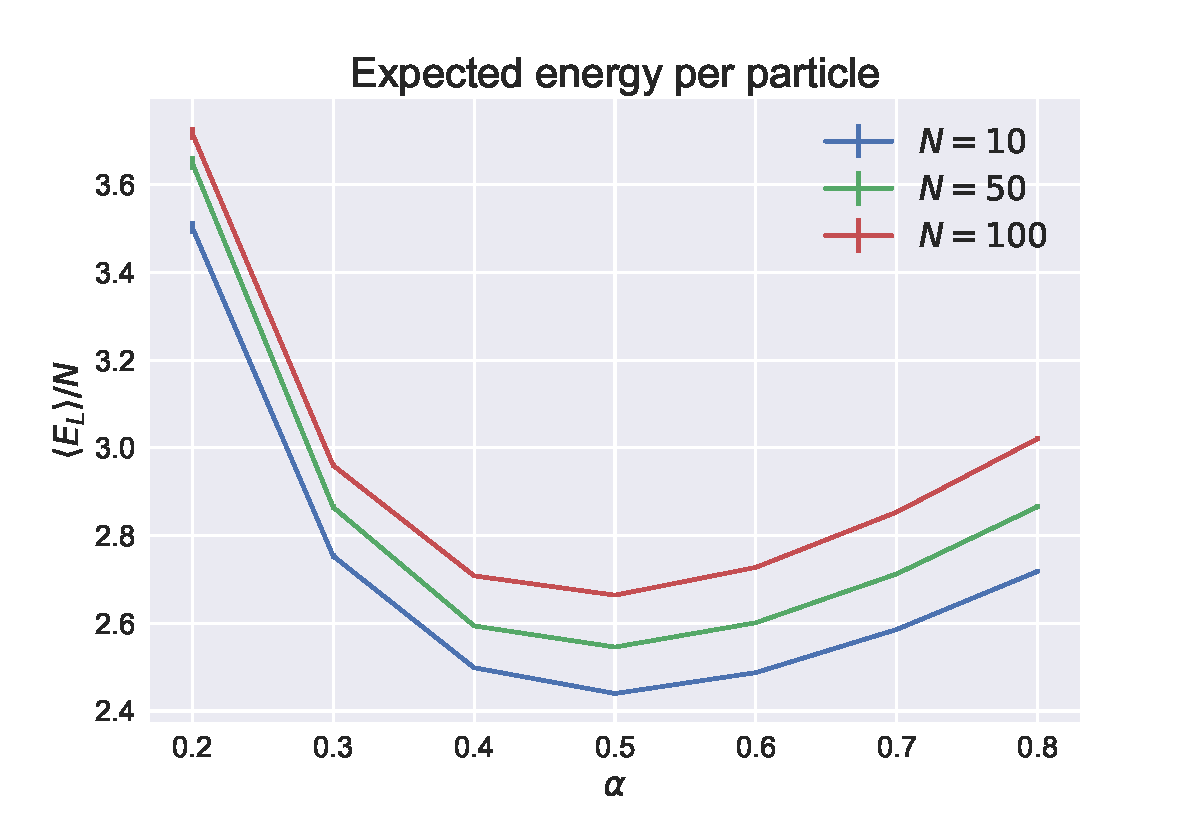
\includegraphics[width=250px]{../data/figures/problem_e.pdf}
             \caption{Local energies as a function of variational parameter $\alpha$
             				 for different number of particles.}
             \label{fig:interacting}
         \end{figure}

\appendix
\section{Brute Force Metropolis-Hastings}

    \begin{figure*}
        \makebox[\textwidth][c]{
            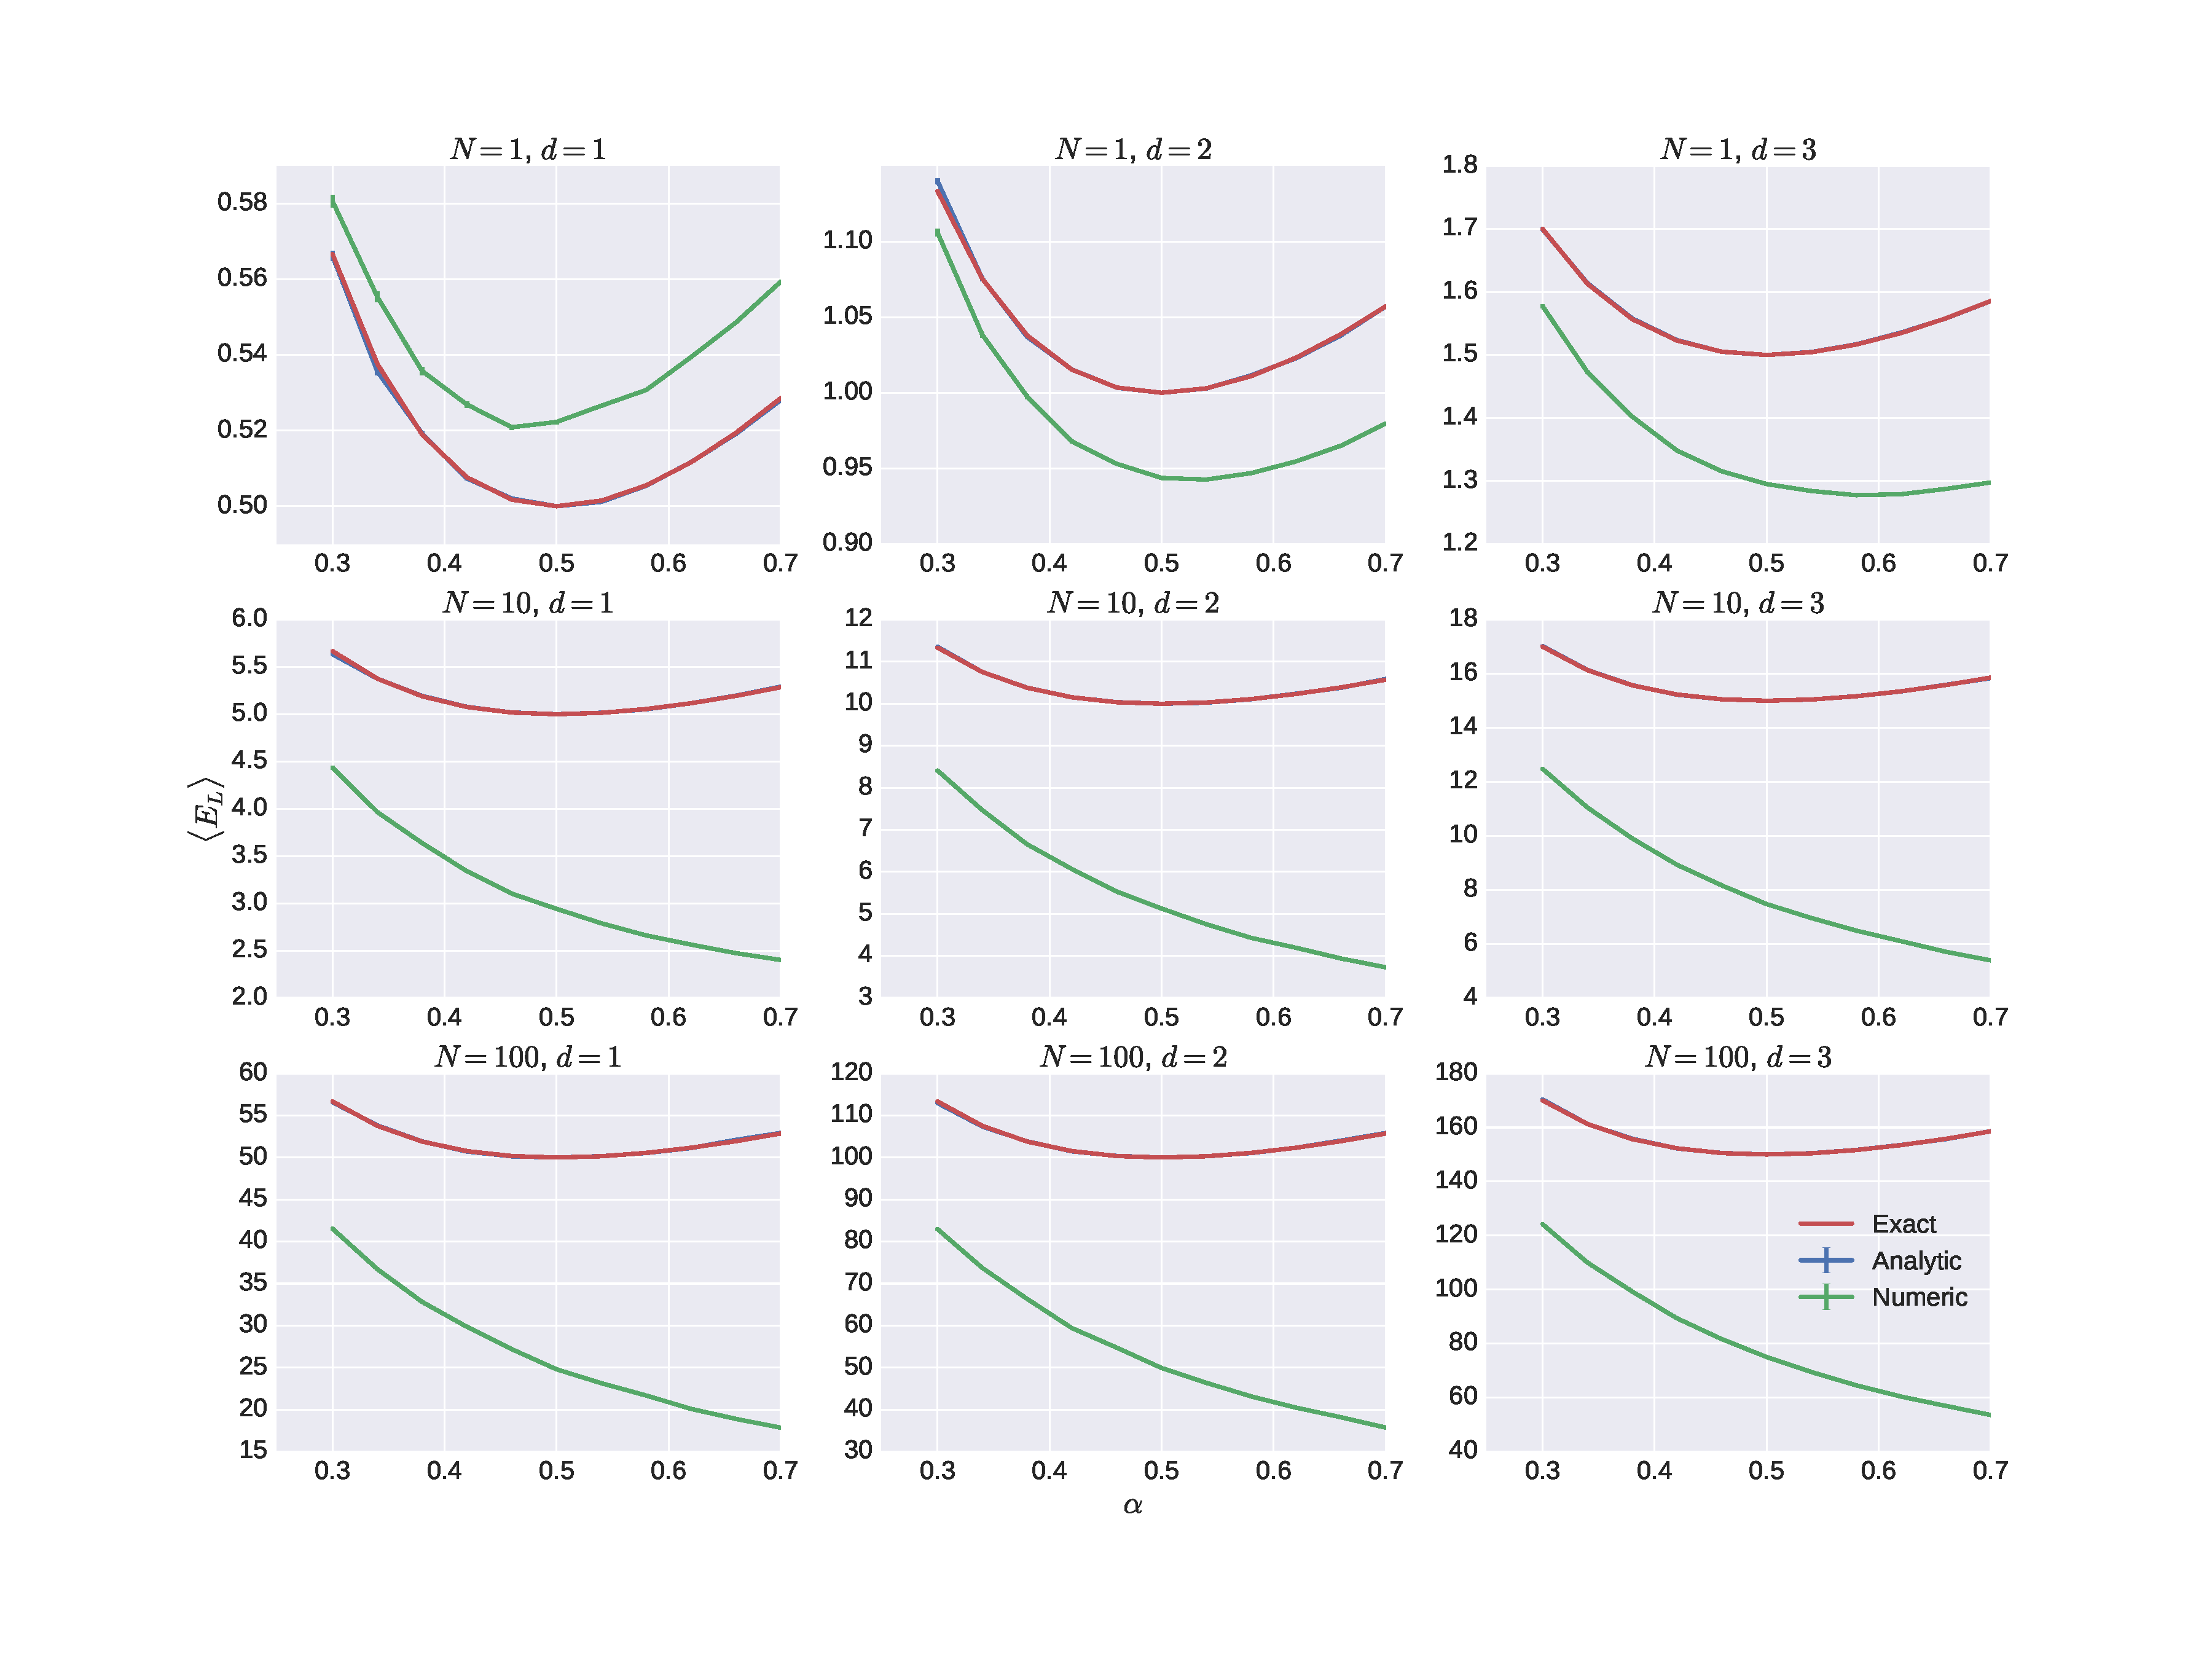
\includegraphics[width=1.2\textwidth]{../data/figures/problem_b.pdf}
        }
        \caption{Comparison of analytic and numeric results with the exact
        expression for the energy as a function of $\alpha$. The plots show the
        standard deviation from the blocking method as error ticks. In the
        figure $N$ is the number of particles and $d$ the number of dimensions.}
        \label{fig:initial_problem_b}
    \end{figure*}


\bibliography{references}



\end{document}
